\documentclass[12pt]{article}
\usepackage[utf8]{inputenc}
\usepackage{booktabs}
\usepackage{geometry}
\usepackage{graphicx}
\geometry{a4paper, margin=1in}
\title{Results of Fisher's Combined Test}
\author{Sara Fraija}
\date{\today}
\begin{document}
\maketitle
\section{Results}

\begin{table}[h!]
\centering
\resizebox{\textwidth}{!}{%
\begin{tabular}{l c c c c c c}
\toprule
\textbf{GRB} & \textbf{Transit} & \textbf{Significance} & \textbf{Corrected Significance} & \textbf{p-value} & \textbf{Corrected p-value} & \textbf{PDF} \\ \midrule
GRB150110923 & 1 & 1.61 & 1.61 & 5.370e-02 & 5.370e-02 & 1.092e-01 \\
GRB150922234 & 1 & 2.31 & 2.31 & 1.044e-02 & 1.044e-02 & 2.768e-02 \\
GRB160726065 & 1 & 0.65 & 0.65 & 2.578e-01 & 2.578e-01 & 3.230e-01 \\
GRB170325331 & 1 & 0.00 & 0.00 & 5.000e-01 & 5.000e-01 & 3.989e-01 \\
GRB180715755 & 1 & 0.58 & 0.58 & 2.810e-01 & 2.810e-01 & 3.372e-01 \\
GRB180718082 & 1 & 1.58 & 1.58 & 5.705e-02 & 5.705e-02 & 1.145e-01 \\
GRB181125371 & 1 & 0.00 & 0.00 & 5.000e-01 & 5.000e-01 & 3.989e-01 \\
GRB190427190 & 1 & 2.55 & 2.55 & 5.386e-03 & 5.386e-03 & 1.545e-02 \\
GRB201008443 & 1 & 2.22 & 2.22 & 1.321e-02 & 1.321e-02 & 3.394e-02 \\
GRB201221963 & 1 & 0.00 & 0.00 & 5.000e-01 & 5.000e-01 & 3.989e-01 \\
GRB210323918 & 1 & 0.66 & 0.66 & 2.546e-01 & 2.546e-01 & 3.209e-01 \\
GRB170817529 & 1 & 2.72 & 2.72 & 3.264e-03 & 3.264e-03 & 9.871e-03 \\
GRB170403583 & 1 & 0.00 & 0.00 & 5.000e-01 & 1.000e+00 & 3.989e-01 \\
GRB170222209 & 1 & 0.68 & 0.00 & 2.483e-01 & 1.000e+00 & 3.166e-01 \\
GRB150922234 & 2 & 1.85 & 1.85 & 3.216e-02 & 3.216e-02 & 7.206e-02 \\
GRB160726065 & 2 & 0.60 & 0.60 & 2.743e-01 & 2.743e-01 & 3.332e-01 \\
GRB170325331 & 2 & 1.00 & 1.00 & 1.587e-01 & 1.587e-01 & 2.420e-01 \\
GRB180715755 & 2 & 0.27 & 0.27 & 3.936e-01 & 3.936e-01 & 3.847e-01 \\
GRB180718082 & 2 & 2.90 & 2.90 & 1.866e-03 & 1.866e-03 & 5.953e-03 \\
GRB181125371 & 2 & 0.98 & 0.98 & 1.635e-01 & 1.635e-01 & 2.468e-01 \\
GRB190427190 & 2 & 0.00 & 0.00 & 5.000e-01 & 5.000e-01 & 3.989e-01 \\
GRB201008443 & 2 & 2.21 & 2.21 & 1.355e-02 & 1.355e-02 & 3.470e-02 \\
GRB201221963 & 2 & 0.75 & 0.75 & 2.266e-01 & 2.266e-01 & 3.011e-01 \\
GRB210323918 & 2 & 0.78 & 0.78 & 2.177e-01 & 2.177e-01 & 2.943e-01 \\
GRB170817529 & 2 & 1.12 & 1.12 & 1.314e-01 & 1.314e-01 & 2.131e-01 \\
GRB170403583 & 2 & 1.59 & 0.51 & 5.592e-02 & 3.044e-01 & 1.127e-01 \\
GRB170222209 & 2 & 2.05 & 1.06 & 2.018e-02 & 1.435e-01 & 4.879e-02 \\
GRB150110923 & 1 & 0.00 & 0.00 & 5.000e-01 & 5.000e-01 & 3.989e-01 \\
\bottomrule
\end{tabular}%
}
\caption{Lista de GRBs con sus Tránsitos, Significancias, Significancias Corregidas, p-values, p-values Corregidos y valores PDF.}
\end{table}


\begin{figure}[h!]
\centering
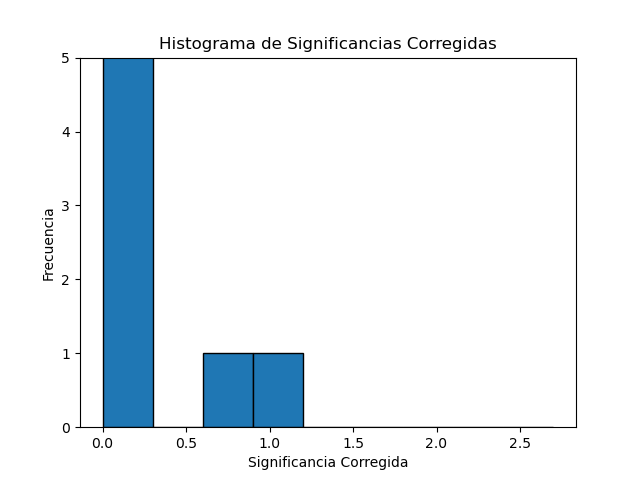
\includegraphics[width=0.45\textwidth]{2nd_Transitcorrected_significance_hist.png}
\hfill
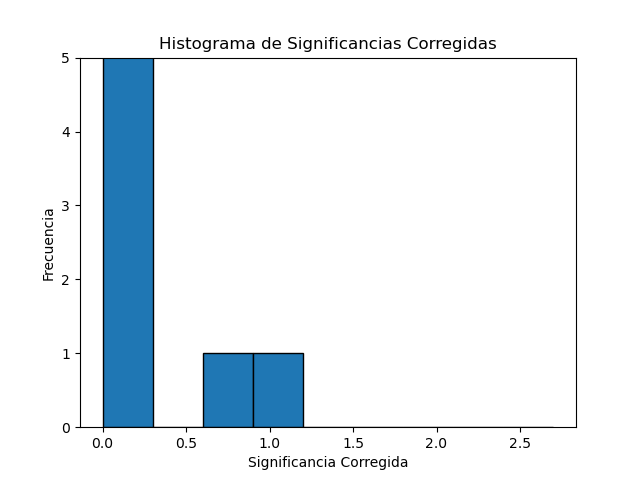
\includegraphics[width=0.45\textwidth]{2nd_Transitcorrected_significance_hist.png}
\caption{Histograma de Significancias (izquierda) y de Significancias Corregidas (derecha).}
\end{figure}


\section*{Conclusion}
Fisher's combined test integrates individual p-values to evaluate a global hypothesis. 
In this analysis, the test statistic obtained was $X^2 = 125.080$ with 56 degrees of freedom. 
For a significance level of 0.05, the critical chi-square value is 74.468. 
Since $X^2$ is greater than the critical value, 
we reject the null hypothesis that the events are independent.
\newline
Additionally, the chi-square value was converted using a normal approximation:
\newline
Normal p-value: 3.922e-07 and Normal significance: 4.94 sigma.


\end{document}
